\documentclass[]{article}
\usepackage{lmodern}
\usepackage{amssymb,amsmath}
\usepackage{ifxetex,ifluatex}
\usepackage{fixltx2e} % provides \textsubscript
\ifnum 0\ifxetex 1\fi\ifluatex 1\fi=0 % if pdftex
  \usepackage[T1]{fontenc}
  \usepackage[utf8]{inputenc}
\else % if luatex or xelatex
  \ifxetex
    \usepackage{mathspec}
  \else
    \usepackage{fontspec}
  \fi
  \defaultfontfeatures{Ligatures=TeX,Scale=MatchLowercase}
\fi
% use upquote if available, for straight quotes in verbatim environments
\IfFileExists{upquote.sty}{\usepackage{upquote}}{}
% use microtype if available
\IfFileExists{microtype.sty}{%
\usepackage{microtype}
\UseMicrotypeSet[protrusion]{basicmath} % disable protrusion for tt fonts
}{}
\usepackage[margin=1in]{geometry}
\usepackage{hyperref}
\hypersetup{unicode=true,
            pdftitle={Guía de trabajos prácticos Bioestadística II: Análisis exploratorio y el primer ANOVA},
            pdfauthor={Derek Corcoran},
            pdfborder={0 0 0},
            breaklinks=true}
\urlstyle{same}  % don't use monospace font for urls
\usepackage{color}
\usepackage{fancyvrb}
\newcommand{\VerbBar}{|}
\newcommand{\VERB}{\Verb[commandchars=\\\{\}]}
\DefineVerbatimEnvironment{Highlighting}{Verbatim}{commandchars=\\\{\}}
% Add ',fontsize=\small' for more characters per line
\usepackage{framed}
\definecolor{shadecolor}{RGB}{248,248,248}
\newenvironment{Shaded}{\begin{snugshade}}{\end{snugshade}}
\newcommand{\KeywordTok}[1]{\textcolor[rgb]{0.13,0.29,0.53}{\textbf{#1}}}
\newcommand{\DataTypeTok}[1]{\textcolor[rgb]{0.13,0.29,0.53}{#1}}
\newcommand{\DecValTok}[1]{\textcolor[rgb]{0.00,0.00,0.81}{#1}}
\newcommand{\BaseNTok}[1]{\textcolor[rgb]{0.00,0.00,0.81}{#1}}
\newcommand{\FloatTok}[1]{\textcolor[rgb]{0.00,0.00,0.81}{#1}}
\newcommand{\ConstantTok}[1]{\textcolor[rgb]{0.00,0.00,0.00}{#1}}
\newcommand{\CharTok}[1]{\textcolor[rgb]{0.31,0.60,0.02}{#1}}
\newcommand{\SpecialCharTok}[1]{\textcolor[rgb]{0.00,0.00,0.00}{#1}}
\newcommand{\StringTok}[1]{\textcolor[rgb]{0.31,0.60,0.02}{#1}}
\newcommand{\VerbatimStringTok}[1]{\textcolor[rgb]{0.31,0.60,0.02}{#1}}
\newcommand{\SpecialStringTok}[1]{\textcolor[rgb]{0.31,0.60,0.02}{#1}}
\newcommand{\ImportTok}[1]{#1}
\newcommand{\CommentTok}[1]{\textcolor[rgb]{0.56,0.35,0.01}{\textit{#1}}}
\newcommand{\DocumentationTok}[1]{\textcolor[rgb]{0.56,0.35,0.01}{\textbf{\textit{#1}}}}
\newcommand{\AnnotationTok}[1]{\textcolor[rgb]{0.56,0.35,0.01}{\textbf{\textit{#1}}}}
\newcommand{\CommentVarTok}[1]{\textcolor[rgb]{0.56,0.35,0.01}{\textbf{\textit{#1}}}}
\newcommand{\OtherTok}[1]{\textcolor[rgb]{0.56,0.35,0.01}{#1}}
\newcommand{\FunctionTok}[1]{\textcolor[rgb]{0.00,0.00,0.00}{#1}}
\newcommand{\VariableTok}[1]{\textcolor[rgb]{0.00,0.00,0.00}{#1}}
\newcommand{\ControlFlowTok}[1]{\textcolor[rgb]{0.13,0.29,0.53}{\textbf{#1}}}
\newcommand{\OperatorTok}[1]{\textcolor[rgb]{0.81,0.36,0.00}{\textbf{#1}}}
\newcommand{\BuiltInTok}[1]{#1}
\newcommand{\ExtensionTok}[1]{#1}
\newcommand{\PreprocessorTok}[1]{\textcolor[rgb]{0.56,0.35,0.01}{\textit{#1}}}
\newcommand{\AttributeTok}[1]{\textcolor[rgb]{0.77,0.63,0.00}{#1}}
\newcommand{\RegionMarkerTok}[1]{#1}
\newcommand{\InformationTok}[1]{\textcolor[rgb]{0.56,0.35,0.01}{\textbf{\textit{#1}}}}
\newcommand{\WarningTok}[1]{\textcolor[rgb]{0.56,0.35,0.01}{\textbf{\textit{#1}}}}
\newcommand{\AlertTok}[1]{\textcolor[rgb]{0.94,0.16,0.16}{#1}}
\newcommand{\ErrorTok}[1]{\textcolor[rgb]{0.64,0.00,0.00}{\textbf{#1}}}
\newcommand{\NormalTok}[1]{#1}
\usepackage{longtable,booktabs}
\usepackage{graphicx,grffile}
\makeatletter
\def\maxwidth{\ifdim\Gin@nat@width>\linewidth\linewidth\else\Gin@nat@width\fi}
\def\maxheight{\ifdim\Gin@nat@height>\textheight\textheight\else\Gin@nat@height\fi}
\makeatother
% Scale images if necessary, so that they will not overflow the page
% margins by default, and it is still possible to overwrite the defaults
% using explicit options in \includegraphics[width, height, ...]{}
\setkeys{Gin}{width=\maxwidth,height=\maxheight,keepaspectratio}
\IfFileExists{parskip.sty}{%
\usepackage{parskip}
}{% else
\setlength{\parindent}{0pt}
\setlength{\parskip}{6pt plus 2pt minus 1pt}
}
\setlength{\emergencystretch}{3em}  % prevent overfull lines
\providecommand{\tightlist}{%
  \setlength{\itemsep}{0pt}\setlength{\parskip}{0pt}}
\setcounter{secnumdepth}{0}
% Redefines (sub)paragraphs to behave more like sections
\ifx\paragraph\undefined\else
\let\oldparagraph\paragraph
\renewcommand{\paragraph}[1]{\oldparagraph{#1}\mbox{}}
\fi
\ifx\subparagraph\undefined\else
\let\oldsubparagraph\subparagraph
\renewcommand{\subparagraph}[1]{\oldsubparagraph{#1}\mbox{}}
\fi

%%% Use protect on footnotes to avoid problems with footnotes in titles
\let\rmarkdownfootnote\footnote%
\def\footnote{\protect\rmarkdownfootnote}

%%% Change title format to be more compact
\usepackage{titling}

% Create subtitle command for use in maketitle
\newcommand{\subtitle}[1]{
  \posttitle{
    \begin{center}\large#1\end{center}
    }
}

\setlength{\droptitle}{-2em}
  \title{Guía de trabajos prácticos Bioestadística II: Análisis exploratorio y el
primer ANOVA}
  \pretitle{\vspace{\droptitle}\centering\huge}
  \posttitle{\par}
  \author{Derek Corcoran}
  \preauthor{\centering\large\emph}
  \postauthor{\par}
  \predate{\centering\large\emph}
  \postdate{\par}
  \date{March 14, 2018}


\begin{document}
\maketitle

{
\setcounter{tocdepth}{2}
\tableofcontents
}
\subsection{Objetivos de este
práctico}\label{objetivos-de-este-practico}

\begin{itemize}
\tightlist
\item
  Entender los supuestos de un ANOVA de una via (independencia,
  aleatoreidad, homocedasticidad y normalidad)
\item
  Entender el concepto de mínimos cuadrados
\item
  Saber cuando realizar un ANOVA e interpretar sus resultados
\end{itemize}

\subsection{Actividad 1 Sueño en
mamíferos}\label{actividad-1-sueno-en-mamiferos}

En esta actividad intentaremos ver si hay diferencias en horas de sueño
en mamíferos por Orden o dieta. Los datos fueron extraidos del trabajo
de Savage and West (2007) y estan incorporados en la base de datos de
\emph{ggplot2} con el nombre de \emph{msleep}, pero estarán en webcursos
en formato csv de todas formas. Para la guía los ejemplos se generarán
en base a la base de datos \emph{InsectSprays} que está en \emph{R} y
que fue extraída de Beall (1942), en la cual se testean la efectividad
de insecticidas en Spray en la abundancia de insectos en plantaciones. Y
en la base de datos \emph{iris} que ya fue entregada, en la que se miden
distintas caracteristicas florales de especies del genero \emph{Iris}
(Anderson 1935).

\subsubsection{Homogeneidad de varianza}\label{homogeneidad-de-varianza}

\paragraph{Inspección visual}\label{inspeccion-visual}

Lo primero que intentaremos explorar de forma visual y a partir de tests
si es que hay homogeneidad de varianza, para esto usaremos boxplots, y
jitter plots, lo cual ya hemos hecho anteriormente:

\begin{Shaded}
\begin{Highlighting}[]
\KeywordTok{ggplot}\NormalTok{(InsectSprays, }\KeywordTok{aes}\NormalTok{(}\DataTypeTok{x =}\NormalTok{ spray, }\DataTypeTok{y =}\NormalTok{ count)) }\OperatorTok{+}\StringTok{ }\KeywordTok{geom_boxplot}\NormalTok{() }\OperatorTok{+}\StringTok{ }\KeywordTok{geom_jitter}\NormalTok{(}\KeywordTok{aes}\NormalTok{(}\DataTypeTok{color =}\NormalTok{ spray)) }
\end{Highlighting}
\end{Shaded}

\begin{figure}
\centering
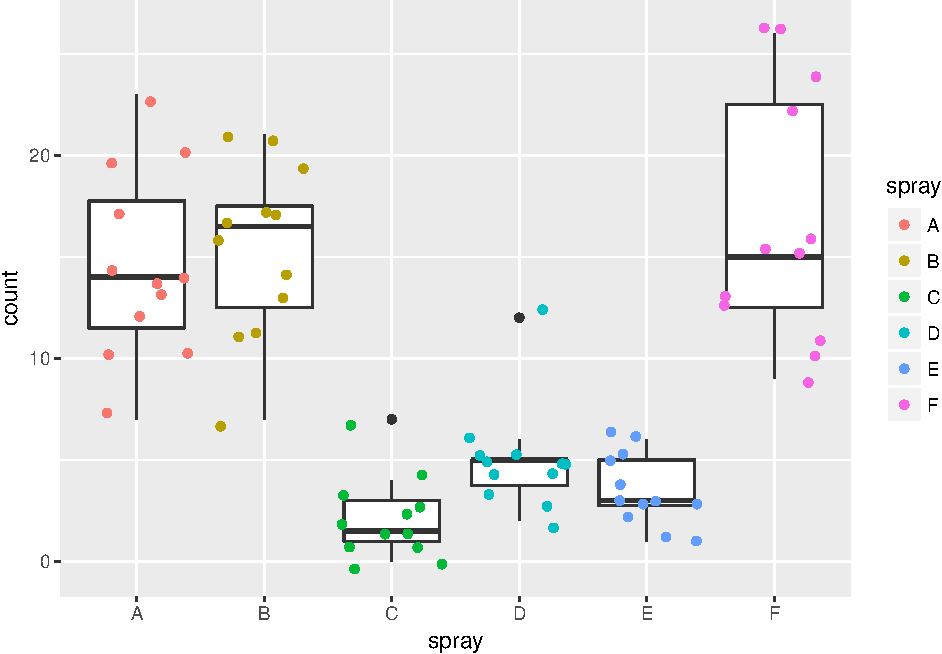
\includegraphics{Guia3_files/figure-latex/unnamed-chunk-1-1.pdf}
\caption{Cuenta de insectos según tipo de insecticida}
\end{figure}

Para explorar visualmente si existe homogeneidad de varianza, se
compraran las cajas y bigotes de los boxplots y se espera que tengan
(Mas o menos distintos tamaños).

\paragraph{Test de Bartlett}\label{test-de-bartlett}

Para realizar un test de homogeneidad de varianza se realiza el test de
bartlett (Bartlett 1937), en este se usa nuestra conocida formula
\emph{y \textasciitilde{} x}, esto es, y explicado por x junto a la
función \emph{bartlett.test}. Para nuestro caso usariamos:

\begin{verbatim}
## 
##  Bartlett test of homogeneity of variances
## 
## data:  count by spray
## Bartlett's K-squared = 25.96, df = 5, p-value = 9.085e-05
\end{verbatim}

Como en este caso, no el valor de p es menor a 0.05, decimos que no hay
homogeneidad de varianza, por lo que no podemos hacer el test.

\subsubsection{Normalidad de los
residuales}\label{normalidad-de-los-residuales}

En el caso de la base de datos \emph{iris}, demostraremos inmediatamente
que si hay homogeneidad de varianza en el ancho del sépalo:

\begin{figure}
\centering
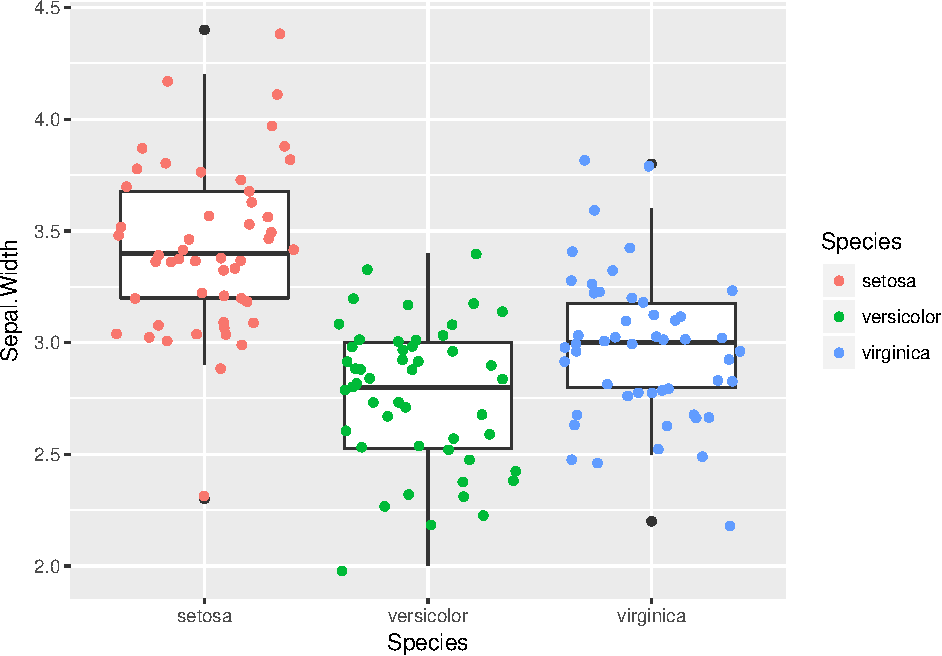
\includegraphics{Guia3_files/figure-latex/unnamed-chunk-3-1.pdf}
\caption{Ancho de sépalo según especie del género Iris}
\end{figure}

\begin{verbatim}
## 
##  Bartlett test of homogeneity of variances
## 
## data:  Sepal.Width by Species
## Bartlett's K-squared = 2.0911, df = 2, p-value = 0.3515
\end{verbatim}

Debido a ello, podemos testar si los residuales tienen una distribución
normalidad de los residuales, para esto lo primero que debemos hacer es
un ANOVA, como fue explicado en el práctico anterior y guardar este
objeto con un nombre:

\paragraph{Extracción de los residuales del
modelo}\label{extraccion-de-los-residuales-del-modelo}

Para exter los residuales, podemos hacerlo de dos formas, si solo
queremos un vector de sus valores, podemos extraelo desde el modelo
mimso utlizando \emph{\$residuals}. Si queremos guardarlo en un
dataframe mas completo podemos utilizar la función \emph{augment} del
paquete \emph{broom}.

La segunda opción nos entregará más información que podremos utilizar
más tarde, pero ambas sirven para testear normalidad, la siguiente tabla
muestra las primeras 6 observaciones generadas por la función
\emph{augment}, donde \emph{resid}, son los residuales.

\begin{longtable}[]{@{}rlrrrrrrr@{}}
\caption{primeras 6 observaciones del dataframe resultante de
augment}\tabularnewline
\toprule
Sepal.Width & Species & .fitted & .se.fit & .resid & .hat & .sigma &
.cooksd & .std.resid\tabularnewline
\midrule
\endfirsthead
\toprule
Sepal.Width & Species & .fitted & .se.fit & .resid & .hat & .sigma &
.cooksd & .std.resid\tabularnewline
\midrule
\endhead
3.5 & setosa & 3.428 & 0.048 & 0.072 & 0.02 & 0.341 & 0.000 &
0.214\tabularnewline
3.0 & setosa & 3.428 & 0.048 & -0.428 & 0.02 & 0.339 & 0.011 &
-1.273\tabularnewline
3.2 & setosa & 3.428 & 0.048 & -0.228 & 0.02 & 0.340 & 0.003 &
-0.678\tabularnewline
3.1 & setosa & 3.428 & 0.048 & -0.328 & 0.02 & 0.340 & 0.006 &
-0.975\tabularnewline
3.6 & setosa & 3.428 & 0.048 & 0.172 & 0.02 & 0.341 & 0.002 &
0.511\tabularnewline
3.9 & setosa & 3.428 & 0.048 & 0.472 & 0.02 & 0.339 & 0.013 &
1.404\tabularnewline
\bottomrule
\end{longtable}

\paragraph{Inspección visual de los
residuales}\label{inspeccion-visual-de-los-residuales}

Existen dos formas de visualizar los residuales para determinar si la
distribución de estos es o no es normal, histogramas y el qqplot.

\subparagraph{Histograma}\label{histograma}

Los histogramas nos darán una representación visual para tratar de
entender si la distribución es normal, para esto, solo necesitamos usar
el comando \emph{hist}, seguido del vector de los residuales, este es el
comando para hacer el histograma con cualquiera de las dos bases de
datos, el resultado debiera ser el mismo:

\begin{Shaded}
\begin{Highlighting}[]
\KeywordTok{hist}\NormalTok{(Residuales)}
\KeywordTok{hist}\NormalTok{(Resultados}\OperatorTok{$}\NormalTok{.resid)}
\end{Highlighting}
\end{Shaded}

\begin{figure}
\centering
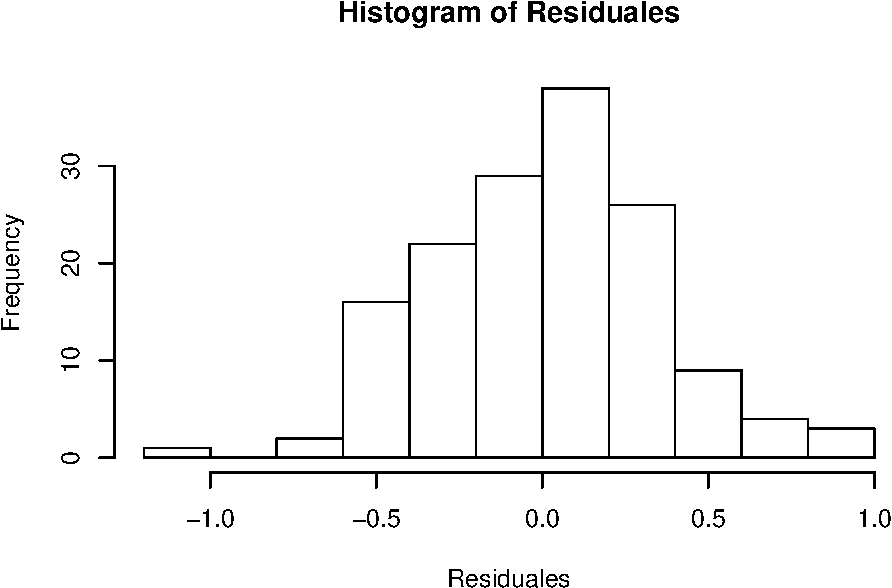
\includegraphics{Guia3_files/figure-latex/unnamed-chunk-9-1.pdf}
\caption{Histograma de los resiudales del modelo ANOVA}
\end{figure}

\subparagraph{QQplot}\label{qqplot}

El qq plot es otra forma visual de establecer si los residuales son o no
son normales, para esto, lo esperado es que la gráfica resultante sea
una diagonal lo mas recta posible, para esto usaremos la función
\emph{qqnorm}, con nuestros residuales, denuevo, podemos usar cualquiera
de las dos versiones de nuestros datos:

\begin{Shaded}
\begin{Highlighting}[]
\KeywordTok{qqnorm}\NormalTok{(Residuales)}
\KeywordTok{qqnorm}\NormalTok{(Resultados}\OperatorTok{$}\NormalTok{.resid)}
\end{Highlighting}
\end{Shaded}

\begin{figure}
\centering
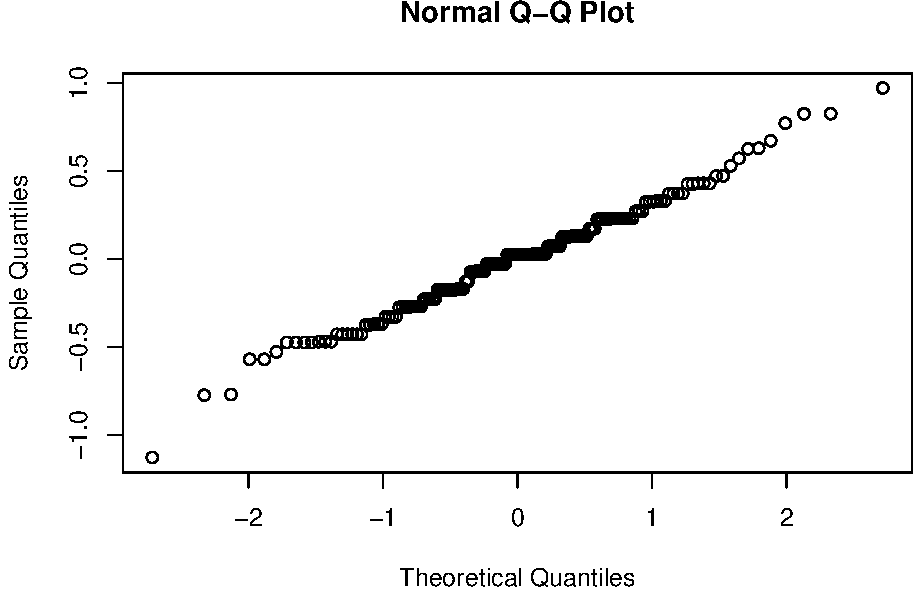
\includegraphics{Guia3_files/figure-latex/unnamed-chunk-11-1.pdf}
\caption{qqplot de los resiudales del modelo ANOVA}
\end{figure}

\paragraph{Test de Shapiro para determinar
normalidad}\label{test-de-shapiro-para-determinar-normalidad}

La forma más sencilla de determinar normalidad es usando el test de
Shapiro-Wilk de normalidad (Royston 1995). Al igual que el test de
Bartlett, si el valor de p es menor a 0.05, determinamos que la
distribución de los datos no son normales, la función en \emph{R} para
este test es \emph{shapiro.test}, y al igual que en los casos anteriores
de \emph{hist} y \emph{qqpot}, solo necesitamos de usar un vector de
residuales para ver el resultado del test. En nuestro caso:

\begin{Shaded}
\begin{Highlighting}[]
\KeywordTok{shapiro.test}\NormalTok{(Residuales)}
\KeywordTok{shapiro.test}\NormalTok{(Resultados}\OperatorTok{$}\NormalTok{.resid)}
\end{Highlighting}
\end{Shaded}

\begin{verbatim}
## 
##  Shapiro-Wilk normality test
## 
## data:  Residuales
## W = 0.98948, p-value = 0.323
\end{verbatim}

Ya que el valor de p es menor a 0.05, podemos decir que la distribución
de nuestros residuales es normal, y por lo tanto el test cumple con los
supuestos, y esto hace que sea valido el ANOVA, por lo que podemos ver
nuestros resultados. La homogeneidad de Varianza es mas importante que
la normalidad de residuales para estos casos, para ejemplos de lo que se
debe hacer si se viola la normalidad ver Lix, Keselman, and Keselman
(1996)

\subsection{Actividad 2 Suma de
cuadrados}\label{actividad-2-suma-de-cuadrados}

Tanto los ANOVAS como las regresiones lineales se basan en minimizar la
suma de cuadrados, es la suma de los cuadrados de los errores o
residuales.

\subsubsection{¿Que es el error? ¿Por qué al
cuadrado??}\label{que-es-el-error-por-que-al-cuadrado}

\begin{figure}
\centering
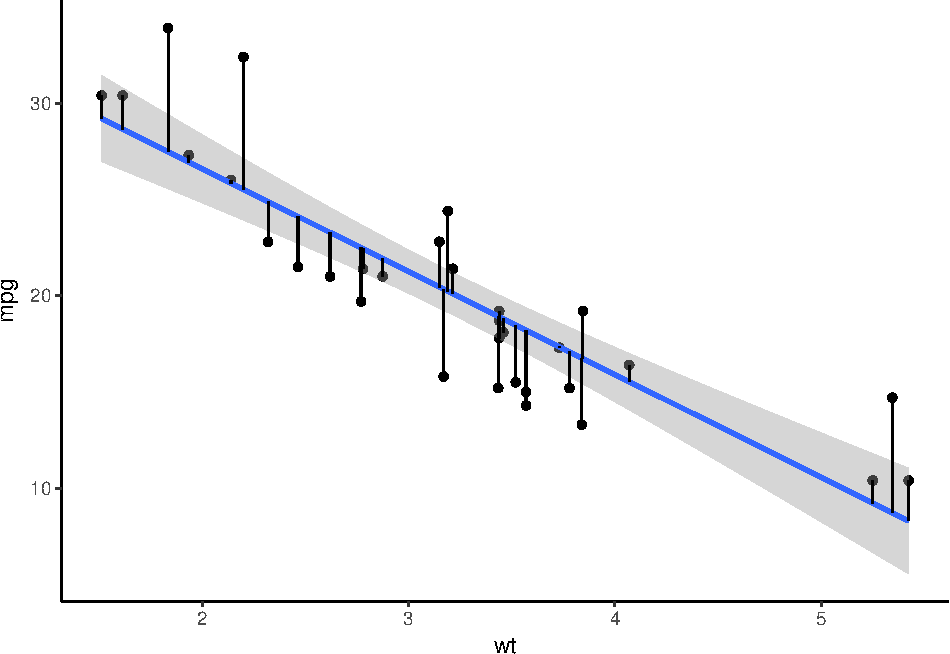
\includegraphics{Guia3_files/figure-latex/unnamed-chunk-14-1.pdf}
\caption{Errores de una regresión lineal ejemplificados con la linea
entre el valor predicho y el observado}
\end{figure}

En la figura y en la formula vemos ejemplificado que es el error,
también conocido como residual, este es simplemente el valor observado

\[Observado - Predicho\]

El objetivo de todo modelo es el de minimizar estos errores, al ajustar
el mejor modelo posible.

Los errores seimpre se calculan al cuadrado, discutiremos por que en
clase

\[\sum_{i=1}^{n} (Observado - Predicho)^2\]

\subsection*{Referencias}\label{referencias}
\addcontentsline{toc}{subsection}{Referencias}

\hypertarget{refs}{}
\hypertarget{ref-anderson1935irises}{}
Anderson, Edgar. 1935. ``The Irises of the Gaspe Peninsula.''
\emph{Bulletin of the American Iris Society} 59: 2--5.

\hypertarget{ref-bartlett1937properties}{}
Bartlett, Maurice S. 1937. ``Properties of Sufficiency and Statistical
Tests.'' \emph{Proc. R. Soc. Lond. A} 160 (901). The Royal Society:
268--82.

\hypertarget{ref-beall1942transformation}{}
Beall, Geoffrey. 1942. ``The Transformation of Data from Entomological
Field Experiments so That the Analysis of Variance Becomes Applicable.''
\emph{Biometrika} 32 (3/4). JSTOR: 243--62.

\hypertarget{ref-lix1996consequences}{}
Lix, Lisa M, Joanne C Keselman, and HJ Keselman. 1996. ``Consequences of
Assumption Violations Revisited: A Quantitative Review of Alternatives
to the One-Way Analysis of Variance F Test.'' \emph{Review of
Educational Research} 66 (4). Sage Publications Sage CA: Thousand Oaks,
CA: 579--619.

\hypertarget{ref-royston1995remark}{}
Royston, Patrick. 1995. ``Remark as R94: A Remark on Algorithm as 181:
The W-Test for Normality.'' \emph{Journal of the Royal Statistical
Society. Series C (Applied Statistics)} 44 (4). JSTOR: 547--51.

\hypertarget{ref-savage2007quantitative}{}
Savage, Van M, and Geoffrey B West. 2007. ``A Quantitative, Theoretical
Framework for Understanding Mammalian Sleep.'' \emph{Proceedings of the
National Academy of Sciences} 104 (3). National Acad Sciences: 1051--6.


\end{document}
